\chapter{算法实现}
本章,我们将从判决预测、关键词抽取、类案搜索等模块来详细介绍项目中用到的算法模型。在模型中,我们统一使用了THULAC进行中文分词,我们使用的词向量是利用FastText模型,在大规模的法律文书语料库上进行的预训练,我们采用的词向量维度为200维。

对于每一个模块,我们将分别从任务的描述定义、算法的创新点、算法模型细节三个方面来进行详细阐述。


\section{背景知识}
\iffalse
\subsection{卷积神经网络}

卷积神经网络(Convlutional Neural Network, CNN)是多层感知机(Multi-Layer Perceptrons, MLP)的变种,由生物学家在早期关于猫视觉皮层细胞的深入研究发展而来,猫视觉皮层的细胞存在一个非常复杂的构造,这些细胞对视觉输入空间的某些子区域非常敏感,称之为感受野。

CNN的本质是一个多层感知机,成功的原因在于它所采用的局部连接和权值共享的方式:1)一方面减少了权值的数量,这样使得神经网络更加容易被优化;2)另一方面它降低了模型的复杂度,即减小了模型过拟合的风险。

这些优点在模型的输入是图片时表现得更加明显,它使得图像可以直接作为网络的输入,避免了传统识别算法中复杂的、耗费大量人力的特征提取和数据重建的过程,因此在CNN在图像的处理过程中具有非常大的优势,因为网络能够自行抽取图像的特征包括颜色、纹理、形状及图像的拓扑结构,在处理二维图像的问题上,特别是识别位移、缩放及其他形式扭曲不变性的应用上具有很强的的鲁棒性和运算效率等

\subsection{网络结构}
卷积神经网络是一种带有卷积结构的深度神经网络,卷积结构可以减少深层网络占用的内存量,其三个关键的操作,其一是局部感受野,其二是权值共享,其三是池化层(Pooling layer),减少了网络的参数数量,缓解了模型的过拟合问题。

卷积神经网络是一种多层的监督学习神经网络,隐含层的卷积层和池采样层是实现卷积神经网络特征提取功能的核心模块。该网络模型通过采用梯度下降法最小化损失函数对网络中的权重参数逐层反向调节,通过频繁的迭代训练提高网络的精度。卷积神经网络的低隐层是由卷积层和最大池采样层交替组成,高层是全连接层对应传统多层感知器的隐含层和逻辑回归分类器。第一个全连接层的输入是由卷积层和子采样层进行特征提取得到的特征图像。最后一层输出层是一个分类器,可以采用逻辑回归,Softmax回归甚至是支持向量机对输入图像进行分类。


\begin{itemize}
	\item \textbf{卷积层(Convolutional layer)}:卷积神经网路中每层卷积层由若干卷积单元组成,每个卷积单元的参数都是经过\textbf{反向传播算法}训练得到的。卷积运算的目的是提取输入的不同特征。
	\item \textbf{线性整流层(Rectified Linear Units layer, ReLU layer)}:使用线性整流作为激活函数。它可以增强判定函数和整个神经网络的非线性特性,而本身并不会改变卷积层。
	\item \textbf{池化层(Pooling layer)}:通常在卷积层之后会得到维度很大的特征,将特征切成几个区域,取其最大值或平均值,得到新的、维度较小的特征。
	\item \textbf{全连接层(Fully-Connected layer)}:完成从输入到标签集的映射,即分类。
\end{itemize}

\begin{figure*}[h]
    \centering
    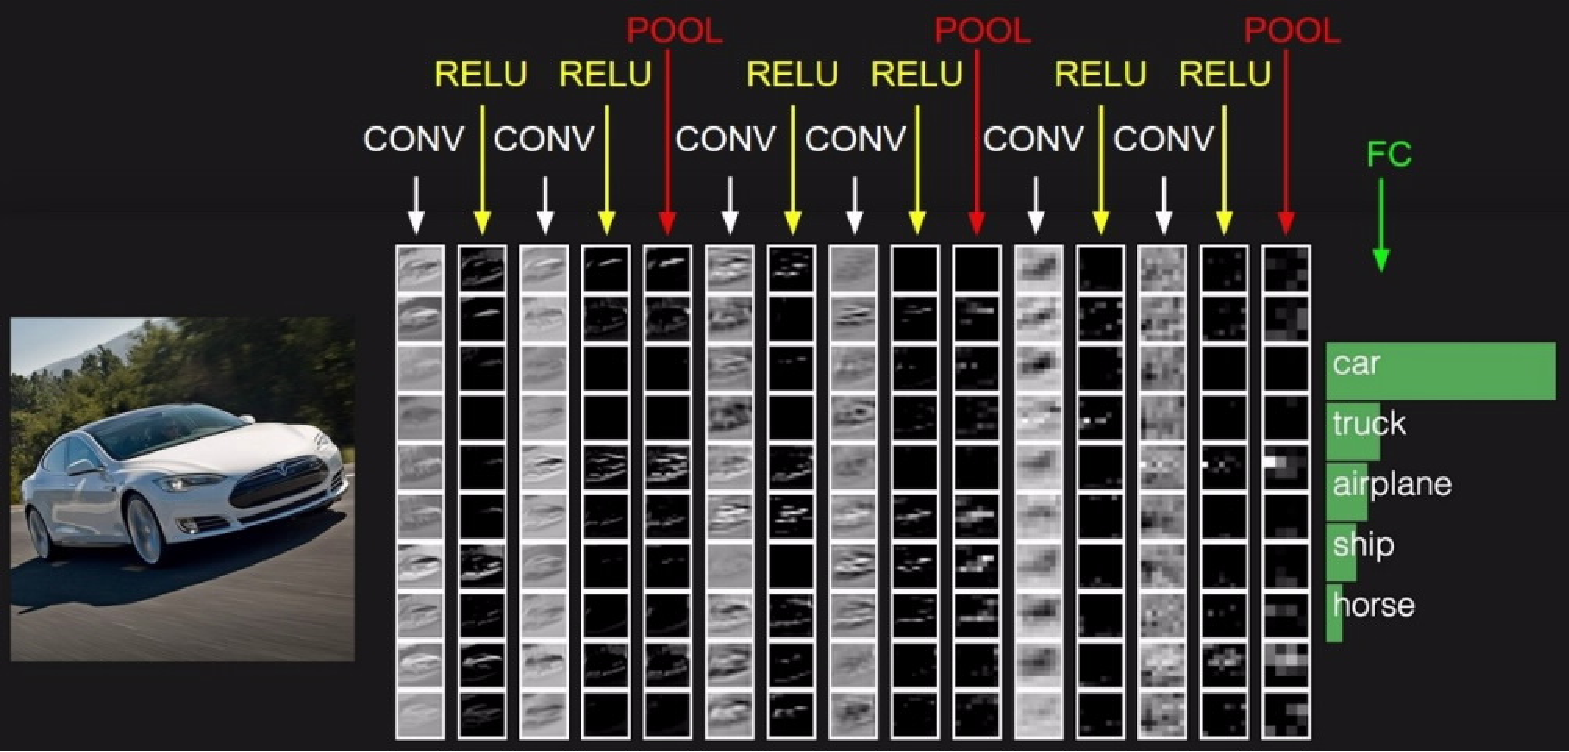
\includegraphics[width=\linewidth]{figures/cnn1}
    \caption{卷积神经网络实例}
    \label{fig:cnn1}
\end{figure*}

图~\ref{fig:cnn1}是一个卷积神经网络各层应用的实例:


卷积神经网络中最基础的操作是卷积。基础 CNN 所用的卷积是一种 2-D 卷积。也就是说,卷积核(kernal)只能在 x,y 上滑动位移,不能进行深度(跨通道)位移。

卷积需要输入两个参数,实质是二维空间滤波,滤波的性质与卷积核选择有关,CNN 的卷积是在一个 2-D 卷积核与 2-D 输入映射之间,在各通道分别完成的。

我们假设单一通道输入的空间坐标为 ${\displaystyle (x,y)}$,kernel 大小是 ${\displaystyle p \times q}$,kernel 权重为 ${\displaystyle w}$,图像亮度值是 ${\displaystyle v}$,卷积过程就是 kernel 所有权重与其在输入图像上对应元素亮度之和,可以表示为:${\displaystyle conv_{x,y} = \sum_i^{p*q}w_i v_i}$。

下面即是一个例子:

\begin{figure*}[ht]
    \centering
    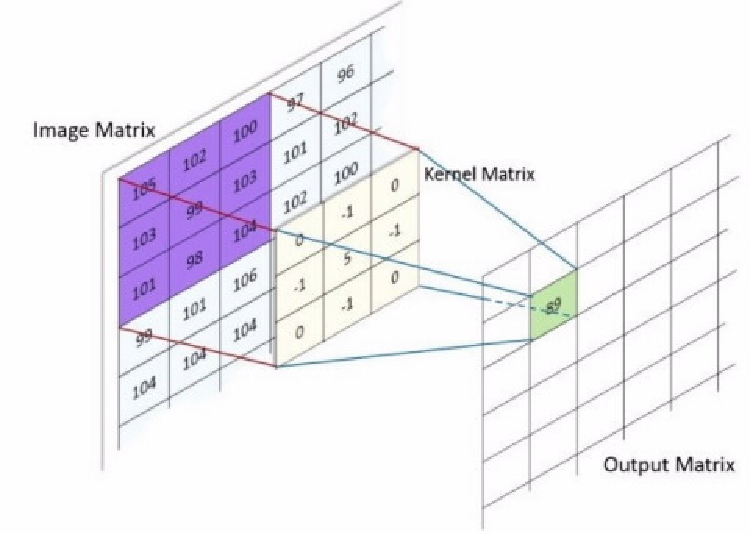
\includegraphics[width=\linewidth]{figures/cnn_conv}
    \caption{卷积层的例子}
    \label{fig:cnn_conv}
\end{figure*}

将 kernel 随 ${\displaystyle (x,y)}$ 平移扫描,即可以得到输出空间。需要特别说明的是,卷积层可能包含多个 kernel,用以抓取多个特征;扫描步长、方向也可能有所不同。

卷积之后,通常会加入偏置(bias),并引入非线性激活函数(activation function),令偏置为 ${\displaystyle b}$,激活函数为 ${\displaystyle h\left(\right)}$,经过激活函数后,得到的结果是 ${\displaystyle z_{x,y}=h\left(\sum_i^{p*q} w_i v_i +b\right)}$。

池化(Pooling)是卷积神经网络中另一个重要的概念,它实际上是一种形式的降采样。有多种不同形式的非线性池化函数,而其中“最大池化(Max pooling)”是最为常见的。它是将输入的图像划分为若干个矩形区域,对每个子区域输出最大值。直觉上,这种机制能够有效地原因在于,在发现一个特征之后,它的精确位置远不及它和其他特征的相对位置的关系重要。池化层会不断地减小数据的空间大小,因此参数的数量和计算量也会下降,这在一定程度上也控制了过拟合。通常来说,CNN 的卷积层之间都会周期性地插入池化层。

池化层通常会分别作用于每个输入的特征并减小其大小。目前最常用形式的池化层是每隔 2 个元素从图像划分出 ${\displaystyle 2\times 2}$ 的区块,然后对每个区块中的 4 个数取最大值。这将会减少 75\% 的数据量。

出现在 CNN 最后的全连接层的主要目的是分类。这与神经网络中的全连接层是相同的。

CNN 网络的训练一般使用反向传播(Back Propagation)算法。同样地,这即是传统神经网络训练的常用算法。


\subsection{长短时记忆网络}

长短时记忆网络(Long short-term memory, LSTM)是一种用于深度学习领域的循环神经网络(Recurrent Neural Network, RNN)架构。与其他神经网络架构不同,LSTM 网络非常适合基于时间序列数据进行分类、处理和预测。

循环神经网络相比全连接神经网络更擅长处理序列数据,与传统神经网络不同,它们是具有循环的网络,这将允许信息持续存在。

咕咕咕,这里有一张图

上图是一个示意图,一组神经网络 A 接收某些输入 ${\displaystyle x_t}$,并输出一个值 ${\displaystyle h_t}$。循环允许信息从网络的一个步骤传递到下一个。

RNN 的重要能力在于它可以将以前的信息连接到当前任务,例如使用先前的视频帧来帮助对当前帧的理解。然而,对于较长距离的历史信息,RNN 仍无法有效地将其利用。

LSTM 相对 RNN 而言解决了长依赖关系学习的问题,能够记住长时间间隔内的信息。通常地,一个 LSTM 单元包含细胞、输入门、输出门和忘记门。其中,细胞(用${\displaystyle C_t}$ 表示)用于记录需要的长时间间隔的信息;输入门、输出门、忘记门具有删除或添加信息到细胞状态的能力,它们被用于维护细胞的状态、控制进出单元的信息流。

下图是一个示意图:

咕咕咕,这里有另一张图
\fi

\subsection{条件随机场}
条件随机场(Conditional random field,CRF)是条件概率分布模型 $P(Y|X)$,该公式表示的是,当给定一组输入随机变量 $X$ 的条件下另一组输出随机变量的值为 $Y$ 的马尔可夫随机场,也就是说 CRF 的特点为假设输出随机变量 $Y$ 构成马尔可夫随机场。

接下来将首先简单介绍以下马尔可夫场,马尔可夫随机场(Markov random field)的一个别称为概率无向图模型(Probabilistic undirected graphical model)。该模型的标准定义为:设有联合概率分布 $P(V)$ 由无向图 $G=(V, E)$ 表示,其中 $V$ 为图 $G$ 中的节点,用来表示随机变量,$E$ 表示图 $G$ 中的边,用来表示随机变量间的依赖关系。如果联合概率分布 $P(V)$ 满足成对、局部或全局马尔可夫性,就称此联合概率分布为概率无向图模型或马尔可夫随机场。

设有一组随机变量 $Y$ ,其联合分布为 $P(Y)$ 由无向图 $G=(V, E)$ 表示。图 $G$ 的一个节点 $v \in V$ 表示一个随机变量 $Y_v$ ,一条边 $e \in E$ 就表示两个随机变量间的依赖关系。

\begin{itemize}
	\item 成对马尔可夫性。$u, v$ 为无向图 $G$ 中的任意两个没有边连接的节点,其他所有节点为 $O$ ,成对马尔可夫性指:给定 $Y_O$ 的条件下,$Y_u$ 和 $Y_v$ 条件独立。
	%\begin{figure*}
	%	\centering
	%	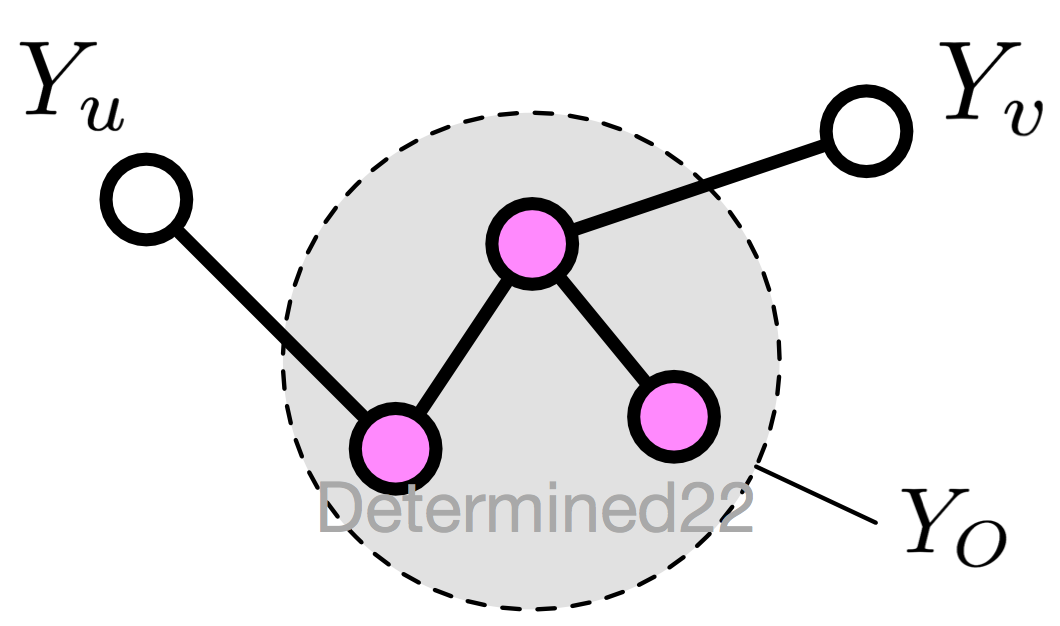
\includegraphics[width=\linewidth/2]{figures/Markov1.png}
    %	\label{fig:Markov1}
	%\end{figure*}
	\begin{equation}
		P(Y_{u}, Y_{v} | Y_{O})=P\left(Y_{u} | Y_{O}\right) P\left(Y_{v} | Y_{O}\right)
	\end{equation}
	
	\item 局部马尔可夫性。设无向图 $G$ 的任一节点 $v$,$W$ 是与 $v$ 有边相连的所有节点,$O$ 是 $v, W$ 外的所有的其他节点,局部马尔可夫性指:给定 $Y_W$ 的条件下,$Y_v$ 和 $Y_O$ 条件独立。
	\begin{figure*}[ht]
		\centering
		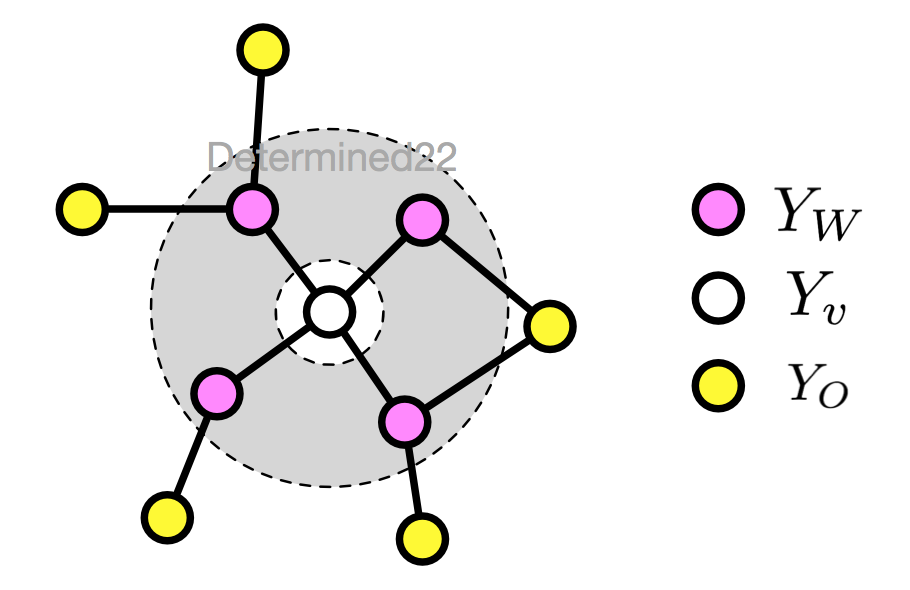
\includegraphics[width=\linewidth/2]{figures/Markov2.png}
		\caption{局部马尔科夫性示意图}
    	\label{fig:Markov2}
	\end{figure*}
	\begin{equation}
		P\left(Y_{v}, Y_{O} | Y_{W}\right)=P\left(Y_{v} | Y_{W}\right) P\left(Y_{O} | Y_{W}\right)
	\end{equation}
	
	\item 全局马尔可夫性。设节点集合 $A,B$ 是在无向图 $G$ 中被节点集合 $C$ 分开的任意节点集合,全局马尔可夫性指:给定 $Y_C$ 的条件下,$Y_A$ 和 $Y_B$ 条件独立。
	\begin{figure*}[ht]
		\centering
		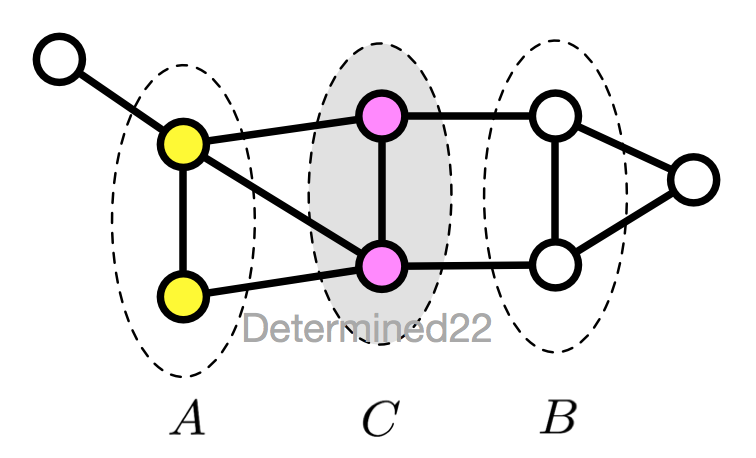
\includegraphics[width=\linewidth/2]{figures/Markov3.png}
		\caption{全局马尔科夫性示意图}
    	\label{fig:Markov3}
	\end{figure*}
	\begin{equation}
		P\left(Y_{A}, Y_{B} | Y_{C}\right)=P\left(Y_{A} | Y_{C}\right) P\left(Y_{B} | Y_{C}\right)
	\end{equation}
\end{itemize}

CRF可以看作是最大熵马尔可夫模型在序列标注问题上的一种推广。这里我们介绍我们平台中用到的用于序列标注问题的线性链条件随机场(linear chain conditional CRF),是根据输入序列来预测输出序列的判别式模型。
	\begin{figure*}[ht]
		\centering
		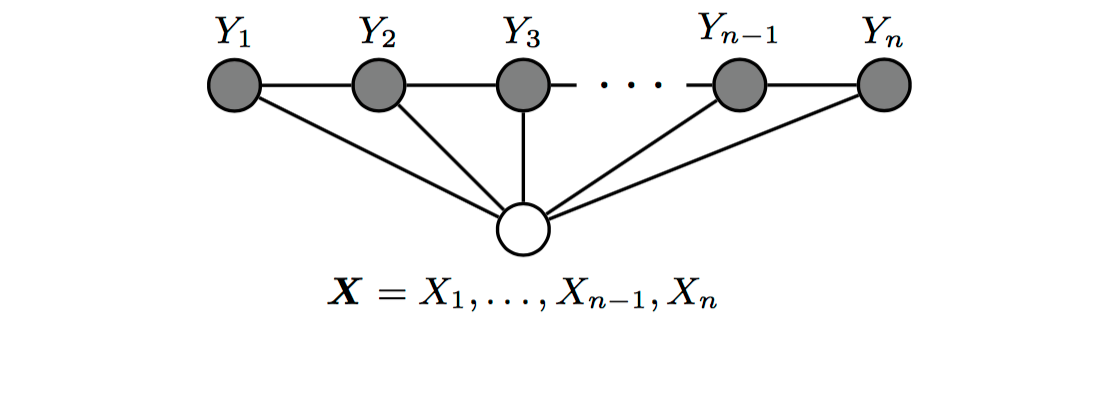
\includegraphics[width=\linewidth]{figures/linear_chain_CRF.png}
		\caption{线性链条件随机场示意图}
    	\label{fig:Markov3}
	\end{figure*}

\begin{equation}
P\left(Y_{v} | X, Y_{w}, w \neq v\right)=P\left(Y_{v} | X, Y_{w}, w \sim v\right)
\label{CRF_11}
\end{equation}

如果随机变量 $Y$ 构成一个由无向图 $G=(V, E)$ 表示的马尔可夫随机场,对任意节点 $v \in V$ 公式\ref{CRF_11}都成立,则称 $P(Y|X)$ 是条件随机场。

对于序列标注问题,$X$ 是需要标注的输入观测序列,$Y$ 是观测序列对应的标记序列(状态序列)。在测试过程,对于给定的观测序列,模型需要求出条件概率最大的输出序列。

其中条件概率被定义为:
%\begin{equation}
	% P(y|x) = \frac{1}{Z} exp\left{(}\sum_{j}\sum_{i=1}^{n-1}\lambda_{j}t_{j}(y_{i+1}, y_i, x, i) + \sum_{k}\sum_{i=1}^{n}\mu_{k}s_{k}(y_i. x. i) \right{)}
	\begin{equation}
P(y | x)=\frac{1}{Z} \exp \left(\sum_{j} \sum_{i=1}^{n-1} \lambda_{j} t_{j}\left(y_{i+1}, y_{i}, x, i\right)+\sum_{k} \sum_{i=1}^{n} \mu_{k} s_{k}\left(y_{i}, x, i\right)\right)
\end{equation}
%\end{equation}
其中,$t_j(y_{i+1}, y_i, x, i)$ 是定义在观测序列的两个相邻标记位置上的转移特征函数,用于刻画相邻变量之间的相关关系以及观测序列对他们的影响。 $s_k(y_i, x, i)$ 是定义在观测序列的标记位置 $i$ 上的状态特征函数,用于刻画观测序列对标记变量的影响,$\lambda_j$ 和 $\mu_k$ 为参数,$Z$ 为规范化因子。模型通过极大似然估计法进行参数训练与优化。

\subsection{Word2vec算法}
Word2vec算法是Google在2013年开源的一个可以将词语映射到低纬向量空间的的算法。该算法就离散的词语转化成连续向量空间中的向量,并可以利用向量之间的关系计算出词语的相似度,同时作为一种词语的表示,word2vec也受到了非常多学者的欢迎。

Word2vec算法中有两类主要模型,分别是 CBOW (Continuous Bag-of-Words Model) 和 Skip-gram (Continuous Skip-gram Model) 模型。两种模型都采用神经网络计算语言模型,结构都大致可分为输入层、投影层和输出层三层结构。

在这里我们重点介绍 CBOW 模型。它是在已知当前词 $x_i$ 的上下文 $\{x_{i−2}, x_{i−1}, x_{i+1}, x_{i+2}\}$ 词向量 $\{w_{i−2}, w_{i−1}, w_{i+1}, w_{i+2}\}$ 的基础上预测当前词 $x_i$ 的词 向量 $w_i$。例如,对于句子 “The quick brown fox jumps over lazy dog” ,预测 fox 这个词时,可以使用 quick、brown、jumps、over 这四个词,它们构成了 fox 的上下文。这样,我们就可以从文本中提取一系列的训练数据。模型得到上下文以后,将这些词的 one-hot 编码累加起来,输入神经网络,然后神经网络进行一些变换,其目标为得到 fox 这个词的 one-hot 编码。训练好之后的神经网络中,隐藏层的权重矩阵就是词嵌入后的向量了。网络结构如图\ref{fig:CBOW}:
\begin{figure*}[ht]
    \centering
    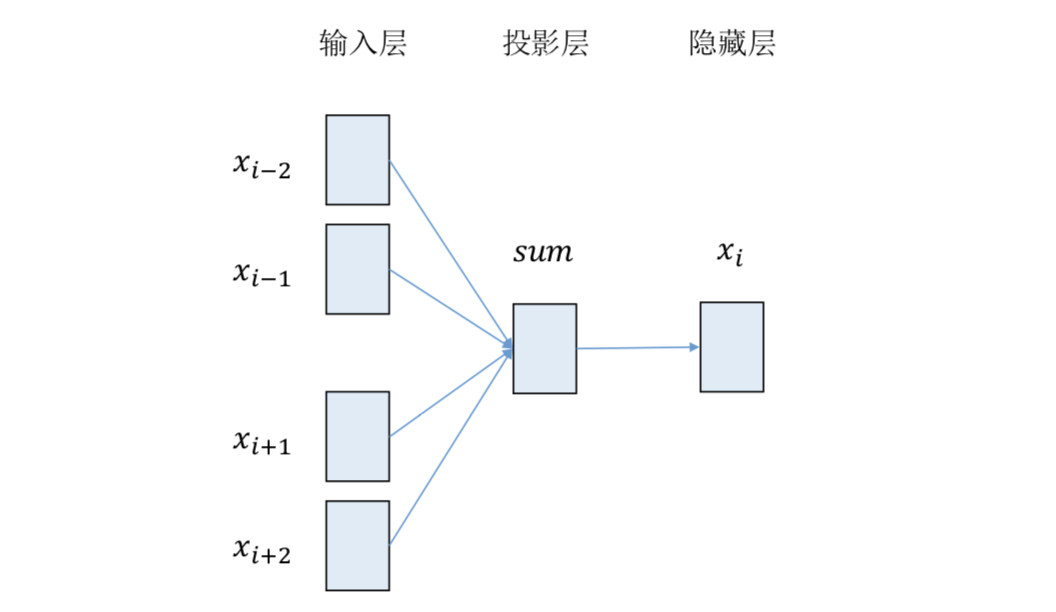
\includegraphics[width=\linewidth]{figures/CBOW.png}
    \caption{CBOW 模型网络结构}
    \label{fig:CBOW}
\end{figure*}

word2vec中CBOW模型大致可分为以下几个部分:
\begin{enumerate}
	\item \textbf{输入层}。包含当前词 $x_i$ 的上下文 $Context(x_i)$ 即包含 $\{x_{i−c},..., x_{i−1}, x_{i+1},..., x_{i+c}\}$ 在内的 $2c$ 个词向量 $\{w_{i−c},..., w_{i−1}, w_{i+1},...,w_{i+c}\}$;
	\item \textbf{投影层}。使用输入层的 $2c$ 个词向量作求和累加,并将其作为下一层的输入,即
		\begin{equation}
			X_{w} = \sum w_{i+j}, j \in (-c,...,-1,1,...,c)
		\end{equation}
	\item \textbf{输出层}。输出层是一颗 Huffman 树。它的叶子节点代表语料中的词语,以每一个词语在数据集中出现的次数作为权重来构建的
\end{enumerate}
对于 CBOW 语言模型,模型的训练目标函数如式\ref{ggg},其中,C 为数据集
中所有词语对应的字典:
	\begin{equation}
		L=\sum_{w \in C} \log (p(w | Context(w)))
	\label{ggg}
	\end{equation}
	
对于这颗最优二叉树,每一个叶子节点即为数据集构成的字典中的某一词语 $w$,对于任一叶子节点必定存在一条路径 $p^w$,从根节点到该叶子节点(且路 径唯一)。路径 $p^w$ 上有 $l_{w} - 1$ 分支,每个分支在进行路径选择时都会产生分类概率,这些选择类似于分类任务。将这些概率累乘起来,就是\ref{ggg}函数中的 $p(w|Context(w))$,具体如下:
	\begin{equation}
		p(w | \text {Context }(w))=\prod_{j=2}^{l w} p\left(d_{j}^{w} | x_{w}, \theta_{j-1}^{w}\right)
	\end{equation}
	
进而二分类函数利用 sigmoid 函数,结合式子\ref{ggg},则最终的目标函数为:
\begin{equation}
L(w, j)=\left(1-d_{j}^{w}\right) \cdot \log \left[\sigma\left(x_{w}^{T} \theta_{j-1}^{w}\right)\right]+d_{j}^{w} \cdot \log \left[1-\sigma\left(x_{w}^{T} \theta_{j-1}^{w}\right)\right]
\end{equation}

其中 sigmoid 函数是神经网络常用的激活函数,式子如下:
\begin{equation}
\sigma(x)=\frac{1}{1+e^{-x}}
\end{equation}

在 word2vec 算法中主要是采用随机梯度上升的方法对目标函数进行优化,不断调整函数中的变量最终达到目标,生成最终的模型。随机梯度上升法的做 法是:每取一组数据 $(w, \text{Context}(w))$,就对目标函数中(相关)参数做一次优化和调整,使其达到局部最大值。在优化的过程中,每一层(主要是三层)参数不断互相影响和优化。通过一定的轮数和目标函数的大小,最终停止优化,生成最后的语言模型。


\section{判决预测}
\subsection{任务描述}
司法的一个重要作用便是对现实生活中发生的各类纠纷、案例以及违法法律的情况进行裁决,而判决就是体现这个裁决的重要场景,而判决结果是每一个案件最关键的基础特征,为了能够直观地捕获到案件的核心特征,在该模块中,\textbf{我们实现了对法学判案要素预测、案件的罪名/案由判断、相关法条推荐、量刑预测功能}。

这四个任务的结果之间具有很强的前后依赖关系,例如,最终量刑强烈依赖于法条的相关规定。在该模块中,四个任务按照顺序构成任务序列,分别对应于模型中$task_{1}$至$task_{4}$。

输入一段文本形式的案情描述,模型通过阅读文本获取其中蕴含的语义信息,将案情映射到高维向量空间,得到一个蕴含关键判案信息的文章向量。在该模块中,我们应用了多任务学习模型(multi-task learning),利用相同的编码器捕获文本信息,通过对每一个任务设置不同的输出层,将高维文本向量映射到不同的输出结果之上。
%再根据不同的任务,将文章向量喂给不同的输出层获得不同的分类结果。

\begin{figure*}[ht]
    \centering
    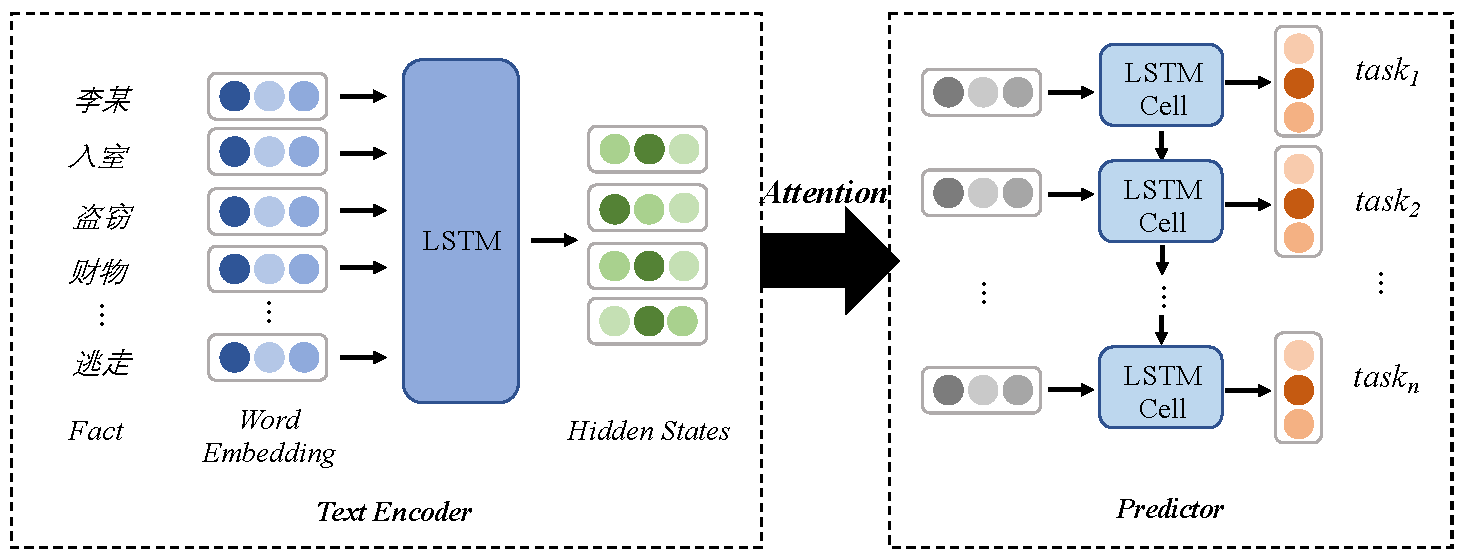
\includegraphics[width=\linewidth]{figures/model1}
    \caption{判决预测模型示意图}
    \label{fig:model1}
\end{figure*}

\subsection{创新点}
我们将上述问题总结为文本分类问题,然而由于无法考虑到在实际法律场景运用中的数据不均衡、相似罪名难以区分等问题,传统文本分类模型在这些任务上无法取得令人满意的效果。通过观察基线模型的预测效果,我们发现了以下现有模型无法解决的难点:
\begin{itemize}
	\item \textbf{数据不均衡(Few-shot)}。在实际场景数据集中,不同案由的案件数量具有极度不均衡性。根据我们对裁判文书网上刑事案件的统计,实际生活中遇到的案件,最频繁发生的十类案件数量(例,盗窃案件、故意伤害案件等)达到了总案件数量的$78.1\%$,然而与此正相反,频率最低的50个罪名案件数量(例,扰乱法庭案、逃税案)只占案件总数量的不到$0.5\%$。以往模型往往关注在高频案件,而忽略了低频案件的判决,然而低频罪名的判决恰恰需要更加大量的法律专业知识。低频罪名的判断也成为提高判决系统稳定性、实用性的关键所在。
	\item \textbf{易混淆罪名难以辨析}。在我国法律体系中存在很多相似的易混淆罪名(例如,盗窃与转化型抢劫、挪用公款罪与贪污罪)。细微的事实改变就可以改变被告罪名判决结果,以往模型在这些罪名上将出现大量的混淆。
	\item \textbf{预测结果矛盾}。传统模型在预测多个任务时,往往因为无法正确捕捉任务之间的依赖关系而预测出矛盾的结果。以往模型往往会预测出完全无关的相关法条、罪名与刑期等,例如模型预测被告为盗窃罪,在刑期上却预测出死刑。预测结果的矛盾导致了以往模型无法运用到实际。
\end{itemize}

在此基础上,我们提出了一个新的判决预测模型,该模型能够捕捉到不同任务之间前后依赖关系,同时通过模拟人类法官判案思路,将判断案件法学要素作为预测判决结果的子任务来提升模型在混淆罪名与低频罪名上的预测效果。综上,我们做出了以下贡献:
% 我们将上述所有功能归纳为文本分类问题,通过观察,上述任务之间有很强的前后依赖关系,例如,相关法条推荐结果往往与罪名及案由预测结果高度相关。并且,根据法学领域从业人员介绍,在实际判案时,大家首先会判断案情中的相关要素,并根据要素判断结果来决定最后的案件的判决。因此,我们有以下创新来提升各个任务的效果:

\begin{itemize}
	\item 提出了一个新的具有高度可扩展性的多任务学习(multi-task learning)模型,相比于以往多任务学习模型,我们的模型可以充分利用各个任务之间的依赖关系,避免了不同任务之间预测结果的矛盾性,同时提升了模型在多个任务的预测效果。
	\item 提出了判决预测新的子任务——判案要素预测,模型通过预测不同案件之间共有的法学要素,来提升模型对法律案件的特征抽取能力。在低频案件的预测上,相比于基线模型,我们的模型实现了超过50\%的效果提升。我们采用了10个最常见的判案要素,如表格\ref{tab:key_elements}所示,要素判断结果可以很好地帮助我们对案件被告涉及罪名做出判断。
	\end{itemize}

\begin{table}[]
\center
\begin{tabular}{l|l}
\hline
\textbf{要素}          & \textbf{要素描述}   \\ \hline
盈利          & 被告犯罪是否以盈利为目的       \\
买卖          & 被告行为中是否涉及买卖行为      \\
死亡          & 被害人是否死亡            \\
暴力          & 被告是否采用了暴力手段犯罪      \\
国家机关/国家工作人员 & 案件中是否涉及国家机关与国家工作人员 \\
公共场合        & 案件是否发生在公共场合        \\
非法占用        & 被告是否以非法占用为目的       \\
伤害          & 被害人是否受伤            \\
主观故意        & 被告主观上是否故意犯罪        \\
生产作业期间      & 案件是否发生在生产作业期间  \\ \hline   
\end{tabular}
\label{tab:key_elements}
\caption{判案要素表}
\end{table}


\subsection{算法模型}
% 算法使用了LSTM作为模型的编码器,使用了全连接神经网络作为输出层。利用了多任务学习的框架,将多个任务进行联合训练得到了效果的提升。
输入案情文本描述后,我们将其进行分词操作将案情描述划分为词语序列$x = \{x_{1}, x_{2}, ..., x_{n}\}$,其中$n$为词语数量。同时,模型适用于multi-task learning任务,我们假设有案件预测结果为$T$,其中$Y = \{y_{1}, y_{2}, ..., y_{|T|}\}$,$y_{i}$为第$i$个子任务的结果。

在该模型中,我们利用长短时记忆网络(LSTM)作为文本编码器,生成案情文本的表示向量。LSTM是循环神经网络的一个变种,通过在每一个循环单元引入输入门、遗忘门、输出门和记忆单元来帮助神经网络捕捉长序列的信息。考虑到我们的输入文本较长,为了捕捉长文本序列关系,我们采用了LSTM作为编码器。编码器结构可分成以下几层。
\begin{itemize}
	\item \textbf{输入层}:文本分词与词向量映射。在获取到输入文本后,我们采用了THULAC作为文本分词器对文本进行分词,同时我们采用了FastText模型在数据集上预训练了词向量。在本层,通过查词向量表,我们将每一个输入单词$x_{i}$转换成词向量$\mathbf{x}_{i}$。此时,输入的文本已经被转换成
	\begin{equation}
		\hat{x} = \{\mathbf{x}_{1}, \mathbf{x}_{2}, ..., \mathbf{x}_{n}\}
	\end{equation}
	\item \textbf{编码层}:为了能够让捕捉到词语序列前后文信息,我们用LSTM对获取到的词向量进行编码处理,获得隐向量序列$\mathbf{h} = \{\mathbf{h}_{1}, \mathbf{h}_{2}, ...,\mathbf{h}_{n}\}$。其中
		\begin{equation}
			\mathbf{h}_{i} = LstmCell(\mathbf{x}_{i}, \mathbf{h}_{i-1})
		\end{equation}
	\item \textbf{注意力层}:我们在循环神经网络基础之上运用了注意力机制(attention)捕获输入文本中的关键信息。通过attention机制,我们可以根据任务的不同,捕获到不同的关键信息,从而为每一个任务都生成一个不同的表示向量$\mathbf{a} = \{\mathbf{a}_{1}, \mathbf{a}_{2}, ..., \mathbf{a}_{n}\}$。其中,$\mathbf{u}^{k}$为每个子任务的表示向量,$\mathbf{W}^{a}$为训练参数。
		\begin{equation}
			\mathbf{a}_{i} = \sum_{j=1}^{n}\alpha_{j}\mathbf{h}_{j}
		\end{equation}
		\begin{equation}
			\alpha_{j} = \frac{exp(tanh(\mathbf{W}^{a}\mathbf{h}_{j})^{T}\mathbf{u}^{k})}{\sum_{t}exp(tanh(\mathbf{W}^{a}\mathbf{h}_{t})^{T}\mathbf{u}^{k})}
		\end{equation}
	\item \textbf{预测层}:在为每一个任务获得其表示向量后,我们利用了LSTM Cell捕捉长序列信息的能力来获取前后任务之间的依赖关系。我们将Attention层的输出当做预测层的输入序列,为每一个子任务初始化一个不同的LSTM单元,从而获取与任务相关的文本表示向量$\hat{\mathbf{ht}}_{i}$。
		\begin{equation}
			\hat{\mathbf{ht}}_{i} = LstmCell(\mathbf{a}_{i}, \mathbf{ht}_{i})
		\end{equation}
		\begin{equation}
			\mathbf{ht}_{i} = \mathbf{W}_{i}\mathbf{ht}_{i-1} + \mathbf{b}_{i}
		\end{equation}
	\item \textbf{输出层}:最后,在获得每一个任务特有的文本表示向量之后,我们采用了全连接神经网络,将包含任务信息的文本向量映射到每个任务相应的分类中。对于每个不同的任务而言,$\mathbf{y}_{i} \in \mathbf{Y}_{i}$,其中$\mathbf{Y}_{i}$是每个任务的分类空间,例如对于罪名预测任务而言,$Y =$\{盗窃罪、抢劫罪……\}
		\begin{equation}
			\mathbf{y}_{i} = softmax(\mathbf{\hat{W}}_{i}\mathbf{ht}_{i} + \mathbf{\hat{b}}_{i})
		\end{equation}
	
\end{itemize}

我们采用了交叉熵损失函数,运用了Adam算法训练模型参数。其中损失函数计算公式如下,
\begin{equation}
	\mathcal{L} = \sum_{j}\mathcal{L}_{j}
\end{equation}
\begin{equation}
	\mathcal{L}_{j}(\hat{\mathbf{y}_{j}}, \mathbf{y}_{j}) = -\sum_{k=1}^{|Y_{j}|}\mathbf{y}_{j, k}log(\hat{\mathbf{y, k}})
\end{equation}

我们将算法运用于判案要素预测、罪名预测、法条预测、刑期预测四个任务上,四个任务的预测结果前后依赖,罪名预测结果依赖于要素预测结果,刑期预测结果与法条内容高度相关。因此,我们将四个任务按照上述顺序构成任务序列,利用任务之间的相关关系,提升各个任务的效果。具体实验结果见章节\ref{cha:result}。


\section{关键词抽取}
\subsection{任务描述}
关键词抽取旨在从信息化的文本中,提取出最重要的成分,通过有限个的关键词,尽可能的还原信息化文本中原本的含义。在传统的数据挖掘中,关键词抽取的方法被用在了各种各样的数据上,提取出的关键词可被用于检索、分类等多种具有实用性的任务中,并起到核心作用。可以说,关键词抽取的技术不仅可以让我们更好的从文本中提取信息,还可以在海量的信息化文本中构建起特征的桥梁。

虽然传统的关键词抽取方法已经被广泛应用,但是它也存在着许多不可避免的问题。在传统方法中,基于词频、词性特征的关键词抽取算法,需要大量的人工介入,在许多领域并不可行,特别是在司法领域。在司法领域中,由于复杂的语言环境、司法化的特有描述、频繁出现的各式各样的人名与地名等因素,现有的所有分词方法均不能很好的处理智慧司法中信息化的文本,因此传统的基于分词的关键词提取技术在司法领域无法发挥很好的效果。

因此,我们提出了一种基于栅栏式长短时记忆神经网络(Lattice-LSTM)的关键词抽取算法。模型在字级别模型框架基础上,融合了所有可能的词语信息,在短文本关键词抽取上模型效果有着显著的提升。

任务输入为一段案情描述的文本,任务的输出为文本中包含的关键词语,这些词语作为文本的法律标签,是用来检索相关案件、法条的重要依据。例如,对于句子:“被告对{\color{red}火灾}发生是否存在{\color{red}过错},应否对原告的合理损失予以{\color{red}赔偿}”中标红的即为关键词,这些关键词可以很好地帮助检索相关法律法规:“关于{\color{red}火灾过错}引发事故责任划分与{\color{red}赔偿}…”。

本模型的训练数据为筛选过后的法律咨询问句,法律文书中的描述案件争议焦点的句子。我们总共整理了10000条待标注数据,通过人工标注的方法,构建了关键词抽取数据集。

在使用时,我们将对每一个句子进行关键词抽取,筛除其中逆文本频率低的词语,将所有句子的关键词进行合并、筛选,得到最终文章级别的关键词。关键词抽取的结果将对后续的相关案例检索提供重要的帮助。

\subsection{创新点}

关键词抽取是自然语言处理领域非常重要的一个任务,提取出的关键词可以用于文本摘要生成、信息检索、问答等下游任务上。传统的关键词抽取算法(TextRank、LDA、TFIDF)已经被应用到许多领域,但是因为其过多依赖于词频、词性等特征而受到文本处理工具效果的限制。

随着深度学习技术的发展,学者提出了许多有监督的关键词抽取算法,在传统基于词频的无监督学习算法的基础上取得了较大的突破。这些模型大体可分为字级别模型与词级别模型。词级别模型与传统无监督学习算法一样,模型依赖于前序分词的效果,导致了最终模型错误的累积。而不少工作已经证明字级别模型因为缺乏词语信息而无法准确抽取文本中关键词。

本项目所要解决的技术问题是:如何提供一种新的不依赖于分词的关键词抽取技术,能够应对智慧司法领域中可能出现的各种输入,例如人名、地名等,做到在复杂的语言环境下提取文本特征,最终提高关键词抽取在智慧司法领域的效果。

团队提出了基于Lattice-LSTM的关键词检索算法,算法在字级别模型的基础上融合了文本中所有可能的词语信息。综上所述,模型有以下创新:
\begin{itemize}
	\item 模型以字模型为基础,将词语的信息有效融入模型中,实验表明,相比于以往关键词抽取算法,模型实现了6\%的效果提升。
	\item 模型充分考虑了文本中所有可能出现的词语的信息,可以有效避免前序步骤分词效果不佳而导致的关键词抽取不准确的缺点。
\end{itemize}

%在早期,大多数人们使用的是基于词频等特征的无监督学习算法,例如TextRank、LDA、TFIDF算法。对于法律这样一个特定领域,关键词抽取的结果往往是一些法言法语,相比于开放领域上的关键词抽取,有着更强的规律性。因此,我们将目前效果最好的命名实体识别算法运用至该任务。同时,由于训练是在句子级别的语料上进行训练,我们设计了筛选算法,将在所有句子上的抽取结果进行合并筛选,得到了一个较好的效果。

\subsection{算法模型}

\begin{figure*}[ht]
    \centering
    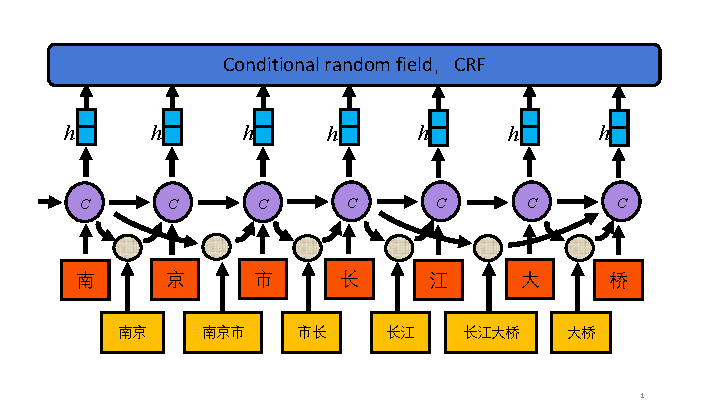
\includegraphics[width=\linewidth]{figures/key_word}
    \caption{关键词抽取模型示意图}
    \label{fig:model2}
\end{figure*}

关键词抽取模型可分为以下几个模块:

\textbf{文本编码模块}。给定待抽取关键词的一个句子实例x,其句子可以拆分为字的序列$\{x_{1}^{c},x_{2}^{c}… x_{L}^{c}\}$,同时连续的相邻几个字还有可能会组成一个词,用$x_{(b,e)}^{w}$表示一个由$\{x_{b}^{c},x_{(b+1)}^{c}… x_{e}^{c}\}$构成的词。我们将句子中包含的字与词的信息${x^{c},x^{w}}$共同作为文本编码模块的输入。具体来看,文本编码模块主要分为输入层和编码层两个层级。
\begin{itemize}
	\item \textbf{输入层}。文本编码模块的输入包含字序列与词信息两部分,输入层的功能就是将输入的字与词转化为对应的低维语义向量。对于字的语义向量,我们从预先在巨大预料库中训练好的BERT模型中提取出字向量,用得到的$k_{c}$维度向量$\hat{x}_{i}$作为对应字的语义表示向量。对于词的向量,我们采用了word2vec在大规模的智慧司法领域语料上提前训练,从而得到了所有词语的$k_{w}$维度向量$\hat{x}_{(b,e)}^{w}$作为对应词语的语义表示向量。这些向量包含了字与词语的语义信息,但是不包含其在具体句子中的上下文相关信息,因此还需要编码层进行进一步编码。
	\item \textbf{编码层}。旨在将输入层处理完的一系列向量通过栅栏式长短时记忆神经网络编码为包含上下文语义的深层语义向量,作为关键词识别模块的输入。
\end{itemize}

接下来我们将详细介绍编码层。在输入层的基础上,我们采用了栅栏式长短时记忆神经网络的结构对字与词的信息进行联合编码。在栅栏式长短时记忆神经网络模型中包含了两种不同的编码单元:词编码单元、字编码单元。

\begin{itemize}
	\item \textbf{词编码单元}。对于输入语句中的每一个可能的词语$x_{(b,e)}^{w}$,都需要经过词编码单元的编码。词编码单元的输入包括要编码的词向量$\hat{x}_{(b,e)}^{w}$、第b个字的字编码单元输出$h_{b}^{c}$和第$b$个字的字编码循环神经元内部表示向量$c_{b}^{c}$,其输出可以定义为:
		\begin{equation}
			\left[
			\begin{array}{c}
				i_{b,e}^{w} \\
				f_{b,e}^{w} \\
				\hat{c}_{b,e}^{w}
			\end{array}
			\right] = 
			\left[
			\begin{array}{c}
				\sigma \\
				\sigma \\
				tanh
			\end{array}
			\right]
			\left(
			W_{\theta}^{w^{T}}
				\left[
				\begin{array}{c}
					\hat{x}_{b,e}^{w} \\
					h_{b}^{c}
				\end{array}
				\right] + b_{\theta}^{w}
			\right)
		\end{equation}
		\begin{equation}
			c_{b,e}^{w} = f_{b,e}^{w} \otimes c_{b}^{c} + i_{b,e}^{w} \otimes \hat{c}_{b,e}^{w}
		\end{equation}
		其中$a \otimes b$表示向量 $a$ 与向量 $b$ 进行对位乘积,$\sigma$表示$Sigmod$激活函数通常被定义为 $\sigma(x)=\frac{e^{x}}{(e^{x}+1)}$,$tanh$表示双曲正切函数,$W_{\theta}^{w^{T}}$和$b_{\theta}^{w}$是模型中的可学习参数,通过前面所述的总体联合学习框架在训练过程中不断更新。这里的词编码单元不直接提供最后的输出,但是其得到的循环神经单元内部表示$c_{(b,e)}^{w}$将会为后面的字编码单元提供原输入语句中词语的信息。由于考虑到了输入语句中出现的每一个可能的词语,模型可以在不依赖于分词的情况下提供词级别的语义信息,从而提升其最终在智慧司法领域的关键词抽取效果。
	\item \textbf{字编码单元}。对于输入语句中的每一个字$x_{i}^{c}$,都需要经过字编码单元的编码。字编码单元的输入包括要编码的字向量$\hat{x}_{i}^{c}$、第$i-1$个字的字编码单元输出$h_{(i-1)}^{c}$和以i结尾的词编码循环神经元内部表示向量$c_{(b,i)}^{w}$,其输出可以定义为:
		\begin{equation}
			\left[
			\begin{array}{c}
				i_{j}^{c} \\
				o_{j}^{c} \\
				f_{j}^{c} \\
				\hat{c}_{j}^{c}
			\end{array}
			\right] = 
			\left[
			\begin{array}{c}
				\sigma \\
				\sigma \\
				\sigma \\
				tanh
			\end{array}
			\right]
			\left(
				W_{\theta}^{w^{T}}
				\left[
				\begin{array}{c}
					\hat{x}_{j}^{c} \\
					h_{j-1}^{c}
				\end{array}
				\right] + b_{\theta}^{c}
			\right)
		\end{equation}
		我们对字进行编码可以得到一个只包含字信息的不完整编码$\hat{c}_{j}^{c}$,为了将词编码单元的输出信息融合进去,还需要在$c_{j}^{c}$的基础上进行一些后继的处理。可以注意到,输入语句中出现的以第e个字结尾的词可能不止一个,例如“桥”、“大桥”、“长江大桥”它们都有相同的结尾,因此需要考虑到不同词对编码信息的贡献,一个词向量对编码的贡献被定义为如下形式:
		\begin{equation}
			i_{b,e}^{c} = \theta
				\left(
					W_{\theta}^{l^{T}}
					\left[
						\begin{array}{c}
							x_{e}^{c} \\
							c_{b,e}^{w}
						\end{array}
					\right] + b_{\theta}^{l}
				\right)
		\end{equation}
		\begin{equation}
			\alpha_{b,j}^{c} = \frac{exp(i_{b,j}^{c})}{exp(i_{j}^{c}) + \sum_{b^{'} \in \{\hat{b}|x_{\hat{b},j}^{w} \in D\}}exp(i_{b,j}^{c})}
		\end{equation}
		\begin{equation}
			\alpha_{j}^{c} = \frac{exp(i_{j}^{c})}{exp(i_{j}^{c}) + \sum_{b^{'} \in \{\hat{b}|x_{\hat{b},j}^{w} \in D\}}exp(i_{b,j}^{c})}
		\end{equation}
		其中$\alpha_{b,j}^{c}$表示从第$b$到第$j$个字构成的词语对当前字编码信息的贡献,$\alpha_{j}^{c}$表示编码信息$c_{j}^{c}$对当前字编码的贡献。通过计算出不同词对当前字的贡献,我们可以加权得到当前字循环神经元内部表示向量$c_{j}^{c}$,具体形式如下:
		\begin{equation}
			c_{j}^{c} = \sum_{b \in \{b^{'}|x_{b^{'},j}^{w} \in D\}}(\alpha_{b,j}^{c} \otimes c_{b,j}^{w} + \alpha_{j}^{c} \otimes \hat{c}_{j}^{c})
		\end{equation}
		通过字编码单元的循环神经元内部表示向量$c_{j}^{c}$,可以得到字编码单元的输出$h_{j}^{c}$,其输出具体定义如下:
		\begin{equation}
			h_{j}^{c} = o_{j}^{c} \otimes tanh(c_{j}^{c})
		\end{equation}
		文本编码模块以一段文本为输入,最终的输出$h_{j}^{c}$即为文本编码模块的输出。输出的向量序列包含了原文中的字语义信息、词语义信息与上下文信息,这些信息将会以低维连续向量的形式传递给关键词识别模块,用于后继的关键词预测功能。
\end{itemize}

\textbf{关键词识别模块}。以文本编码模块的输出为输入。对于一段长度为$L$的文本,文本编码模块会输出一段长度为$L$的向量序列$h_{i}^{c}$,而关键词识别模块则会将这些输入的特征序列,建立条件随机场模型,通过求解模型的最优解作为关键词识别模块的输出。其中条件随机场模型可以表达为以下形式:对于一系列输入$s=h_{1}, h_{2}, …, h_{L}$以及一段预测序列$y=l_{1},l_{2}, …, l_{L}$,定义条件概率$P_{\theta}(y|s)$表示给定输入为$s$的情况下$y$是输入序列$s$的正确预测输出的概率,具体形式如下
	\begin{equation}
		P(y|s) = \frac{exp(\sum_{i}(W_{\theta}^{l_i}h_{i} + b_{\theta}^{l_{i-1},l_{i}}))}{\sum_{y^{'}exp(\sum_{i}(W_{\theta}^{l_{i}^{'}}h_{i} + b_{\theta}^{(l_{i-1}^{'},l_{i}^{i})}))}}
	\end{equation}
	这里的$y'$表示任意预测序列,$W_{\theta}^{l_{i}}$和$b_{θ}^{(l_{(i-1)},l_{i})}$是模型中的可学习参数,在训练过程中这些参数将会不断进行更新。对于上述的条件随机场模型,我们使用维特比算法可以寻找到$y_pred$使得$P(y|s)$达到最大,而寻找到的$y_pred$即是关键词识别模块的最终输出。在最终的输出$y_pred = l_{1},l_{2}, …, l_{L}$中,$l_{i}$有四种可能的取值:(1)非关键词,(2)关键词的第一个字,(3)关键词中间的某个字,(4)关键词的最后一个字。可以根据关键词识别模块的输出,从输入文本中选取子序列作为关键词抽取的结果,从而达到不依赖于分词的关键词抽取。
	
	与现有技术相比,我们提出了一种基于栅栏式长短时记忆神经网络模型的法律文本关键词抽取系统,通过在基于字的预测模型中引入词的语义信息,让模型可以在不依赖分词的情况下同样可以获取到词的语义信息,从而提升模型的稳定性,丰富了关键词特征抽取的细节,实现了关键词抽取算法在智慧司法领域的性能提升,具有良好的实用性。

%该算法将目前前沿的命名实体识别算法——Lattice LSTM,通过将句子拆分成字级别,对每一个字一个标签,来判断最终关键词的范围。在传统的基于字级别的模型基础上,加入词级别信息,这样克服了字级别信息不足、词级别过度依赖于分词效果的缺陷。

%1)	利用n-gram、分词信息等特征为句子中每一个字进行编码,形成字级别特征;

%2)	利用好BiLSTM-CRF的框架,通过BiLSTM对字特征进行编码,再通过CRF捕捉序列信息,进行序列标注;

%3)	改造字级别的LSTM模型,将字与字之间匹配成的所有的可能词的特征融合到LSTM的信息传递中,得到一个Lattice-word model;

%4)	对每个字预测BIE标签,其中B为begin、I为in、E为end;得到最后序列标注的结果。



\section{类案搜索}
\subsection{任务描述}
该模块实现了相关案例推荐的功能。该功能的实现主要基于上述两个模块的模型。该任务模型以案情描述作为输入,通过关键词标签抽取,检索到一批与该案情相似的法律文书,再利用判决预测模块得到的文本向量,对检索到的文书进行重排序,输出一个按照相似度递减的法律文书集合。

\subsection{创新点}
该任务所用算法与传统的搜索引擎算法不同,传统搜索引擎将检索文本与数据库文本进行比对,进而检索出相似度高的文本段。在我们算法中,我们通过抽取出的关键词标签来初步确定相关的文章的集合,再通过判决预测模块中获得的包含文本语义的向量,来对相关集合进行重排序,得到在语义层面相似度最高的文章。

这样的做法改善了传统搜索引擎只关注文本相似度的缺点,通过捕捉语义信息检索以满足用户需求。

综上,我们所要解决的技术问题是:
\begin{itemize}
	\item 提供一种结合语义和语法的信息检索框架,使得我们能够在类案匹配的问题上,能够综合文书的语义和语法来进行相似度的计算一次来提升类案匹配的效果。
	\item 此外,由于文书数据的量及其庞大,我们还需要设计一套能够快速从高维空间找出近邻点的算法,以此来提升类案匹配算法的效率。
\end{itemize}
与现有技术相比,团队提出了一种基于语法表示和语义表示的类案匹配模型。与传统的信息抽取的方法相比,我们将语义信息和语法信息进行了综合的考虑和计算,这使得我们的方法较传统方法在类案匹配的任务上能够有更好的效果。此外,使用多探头的局部敏感度哈希方法,使得我们在类案匹配的时候不会被词语的使用所限制,也能够进一步加速我们的类案匹配系统。

\subsection{算法模型}
团队提供了一种将深度语言模型和传统词法分析相结合的特征抽取和匹配算法,包括如下部分:
\subsubsection{语法表示模型}
为了实现类案匹配的算法,我们需要对每篇文书抽取他们的特征。我们抽取的特征为了涵盖语义的信息,我们必须同时抽取文书在语法上的特征和语义上的特征,所以我们的第一步便是设计一个语法表示的模型来抽取文书的语法特征。

通常情况下,文书的语法特征往往可以由他的用词、用句和某些书写的习惯上来得到,所以我们选取了词频——逆词频的方法来提取文书的语法特征。具体来说,对于一篇文书,我们可以假设:
	\begin{equation}
		d = (w_1,w_2,⋯,w_n)
	\end{equation}
	
其中$d$为文书而$w_1,w_2,⋯,w_n$代表这文书从头至尾的$n$个词,那么我们可以定义在所有文书上的词的集合为:
	\begin{equation}
		W = {w_i |\forall d∈D,w_i∈d}
	\end{equation}
	
其中$D$为所有文档的集合,即遍历所有文书求到所出现词语的并集。那么对于每一个词(比如你好、中国等等),我们可以为这个词定义属于这个词的专属特征。设我们现在想要考察的词为$w$,那么我们可以定义词$w$在文档$d$中的词频为$w$在文档$d$中的出现次数,表示为:
	\begin{equation}
		tf_{w,d} = \frac{n_{w,d)}}{\sum_{w^{'} \in W}n_{w^{'},d}}
	\end{equation}

其中$n_{w,d}$代表词$w$在文档$d$中出现的次数。该式子对词$w$出现的次数做了归一化处理,这是为了使得我们最后的结果在不同文档上拥有同样的表示分布。这样我们便可以衡量一个词在文档中出现的频率,从而拥有了第一个用词的特征。

此外,为了验证一个词的重要程度,我们还需要检查这个词在所有文档中出现的频率。我们定义一个词的逆文档评率为:
	\begin{equation}
		idf_{w}=log⁡ \frac{|D|}{|{d|w \in d}|}
	\end{equation}
	
即该词$w$出现的文档占总文档数量的比例,这样我们可以从另一个层面上反应出一个词的重要程度。有了这两个关于词语的特征后,我们可以定义词$w$在文档$d$中的表示为:
	\begin{equation}
		tfidf_{w,d} = tf_{w,d} \times idf_{w}
	\end{equation}
	
这样我们便可以得到一个词语在一篇文档中的词法表示,从而我们可以得到文档$d$的语法向量表示为:
	\begin{equation}
		v_{d}=(tfidf_{w_{1},d},tfidf_{w_{2},d},⋯,tfidf_{w_{|W|},d})
	\end{equation}
	
即我们可以将所有的词的向量表示进行拼接来得到文档$d$的语法表示$v_{d}$。除此之外,我们需要注意到该向量的长度是非常长的,和$|W|$的大小一致,但这显然是过于巨大,我们不能接受。为了能够让这个向量表示能够应用到实际的类案匹配中,我们通过主成分分析法来对$v_{d}$进行降为处理。即通过所有的向量数据,我们学习一个降维参数$W_{1} \in R^{|W| \times x_{1}}$来抽取对于文本来说最重要的词语句法信息,即我们最终的向量表示因为:
	\begin{equation}
		v_{d}^{'}=v_{d} \times W_{1}
	\end{equation}

其中$x_{1}$为我们降维之后的向量长度。

\subsubsection{语义表示模型}
有了文书关于语法的向量表示之后,我们需要一个能够理解并掌握文书文本深度语义信息的模型,并让该模型抽取出文本深层的含义的向量表示,从而辅助我们完成类案匹配的方法,为了完成这一点,我们采用了深度双向转化编码器来进行语义模型的学习。

具体来说,我们的模型的输入仍然是$ d=(w_1,w_2,⋯,w_n) $即我们的文本信息,我们首先使用词向量编码层对所有的词语进行编码,即我们有:
	\begin{equation}
		d_{vec}=(emb(w_{1}),emb(w_{2}),⋯,emb(w_{n}))
	\end{equation}
	
其中$emb$为我们的词向量编码层,该编码层的参数会在整个训练过程中不断发生变化以此来起到自适应语言模型的作用。对于$emb(w)$,编码层会把我们输入的词编码成一个$x_{emb}$维度的向量,即我们对整个文档使用词向量编码层进行编码之后得到的向量应该满足:$d_{vec} \in R^{n \times x_{emb}}$。

在完成了对于词级别的编码之后,我们便要考虑进一步的对编码出来的矩阵进行编码。为了能够准确的让模型学习到语义的信息,我们在词语编码器之后连续接入$L=12$层的双向转换编码器来解决该问题。对于每一层的双向转换编码器,假设其输入为$x$,那么我们首先使用一个多头的注意力脊椎对其进行编码,即我们有:
	\begin{equation}
		x^{'}=(head_{1},head_{2},⋯,head_{n})
	\end{equation}
	\begin{equation}
		head_{i} = Attention(xW_{Q},xW_{K},xW_{V})
	\end{equation}
	
其中$Attention(xW_{Q},xW_{K},xW_{V})$为在这三者之间进行注意力机制的计算,$W_{Q},W_{K},W_{V}$均为模型中可以学习的参数。此外,注意到我们的模型的深度是非常深的,所以我们需要引入残差网络来避免网络中因为模型深度过深所导致的梯度消失,即:
	\begin{equation}
		x_{out} = x + x^{'}
	\end{equation}

我们重复使用该模型$L$次,便可以得到我们最终的文书$d$的语义表示向量$z_{d}$

除此之外,我们要注意到上述我们描述的只是一个文书的语义表示模型的编码部分,我们需要有优化的目标来让我们的模型从无标注的文书中学习到语言和语义,并将其进行特征化的表示。为此,我们需要设计与之对应的训练任务来帮助模型进行学习。

我们在所有的法律文书上设计了如下两个任务来帮助我们的模型学习到文书的语义信息。我们的第一个任务为给定文书中的两句话,让模型判断这两句话是否为连续的上下文。这样的一个任务能够让模型充分学习到模型的上下文的语义信息,帮助模型从整体上更好地理解文档。我们的第二个任务是我们会在处理文书数据的时候随机地将文书中的部分词语隐去,或者随机替换为其他出现过的词,并要求模型检查以及修改这些被替换的词,进行纠错。这样的一个任务能够让模型更加了解词语的在句子和文档之中扮演的是什么样一个成分,能够让模型更加了解每个词语的意思,也能够让模型更好地区分不同的词在文章中所表达的意思。结合这两个任务,我们成功地训练了我们在法律文书上的语义表示抽取模型,并成功得到了每篇文书的语义表示$z_{d}$。

\subsubsection{特征匹配模型}
在有了前面的两组向量表示$v_d,z_d$之后,我们可以令我们最终文档d的向量表示为
	\begin{equation}
		x_{d}=(v_{d}, z_{d})
	\end{equation}

对于类案匹配的任务,我们实际上希望我们能够通过给定的描述的向量表示$x$,找到$k$个文档使得这$k$个文档的向量表示与$x$的距离尽量小,即我们想要求:
	\begin{equation}
		arg⁡min⁡ max_{|S|=k}⁡\{dis(x,x_{d})|d \in S\}  
	\end{equation}

其中$dis(x,x_d)$为距离函数,我们这里使用欧几里得距离定义我们的距离函数即我们有:
	\begin{equation}
		dis(a,b)=|a-b|_{2}^{2}
	\end{equation}

如果直接遍历所有文档求得与输入文档最相似的k个向量表示所需要的时间显然为$O((k+d)|D|)$,这个值过于巨大我们不能接受。为了加速类案的搜索过程,我们采用局部敏感度哈希算法来完成这个任务。我们选取$r$个哈希函数$(h_1,h_2,⋯,h_r)$,其中$h_i=(a_i,b_i,c_i)$。这里,$a_i$为一个维度与$x_d$一致的一维向量,而$b_i,c_i$为常实数。则我们对文档表示$x_d$的哈希函数为:
	\begin{equation}
		h_{i}(x_{d}) = \left\lfloor \frac{ax+b}{c} \right\rfloor
	\end{equation}
	
由局部敏感度哈希的假设我们有:
	\begin{equation}
		\forall dis(x_{1},x_{2} ) \leq \epsilon, \Pr⁡[h_{i}(x_{1}) = h_{i}(x_{2})] \geq c_1
	\end{equation}
	\begin{equation}
		\forall dis(x_{1},x_{2} ) > t_\epsilon, \Pr⁡[h_{i}(x_{1}) = h_{i}(x_{2})] \leq c_2
	\end{equation}

即任何相似的点都有大概率拥有相同的哈希值,而任何距离较远 的向量的哈希值表示只有小概率是相同的。基于局部敏感度哈希的这个性质,我们可以找到在$r$个哈希函数中与输入文档被哈希到同一个槽位的文档,然后从这里面找到$k$个与输入文档最为相似的文档。用数学化的表示即为:
	\begin{equation}
		D^{'}=\bigcup_{i=1}^{r}\{d|h_{i}(x)=h_{i}(d)\} 
	\end{equation}
	\begin{equation}
		S^{'} = argmin \max_{|S|=k,S \subset D^{'}}\{dis(x,x_d)|d \in S\}
	\end{equation}

即我们通过局部敏感度哈希的方法将我们需要搜索的解空间大大减小,缩小至$D^{'}$的范围。但是这种方法仍然存在一种弊端,即为了达到一个较高的准确率,我们往往需要一个稍大的$ r $即哈希函数的个数来保证我们不会有所遗漏,这个$r$的取值往往会大于$100$,而我们的文档数量是千万级别的,这样的存储量使我们所无法接受的。为此,我们采用多探头的局部敏感度哈希算法,即我们基于局部敏感度哈希的另外一个假设:
	\begin{equation}
		\forall dis(x_{1},x_{2}) \leq \epsilon, \Pr⁡[|h_i(x_1 )-h_i(x_2 )| \leq \alpha ]\geq c_1
	\end{equation}
	
即相似的向量的哈希值表示的距离不会特别大,由此我们可以在哈希出来的值$h_i(x)$的空间附近进行广度搜索,将一个范围内的答案全部纳入考虑,即我们有:
	\begin{equation}
		D^{'}= \bigcup_{i=1}^{r}\{d| |h_i(x)-h_i(d)|\leq \alpha\} 
	\end{equation}
	\begin{equation}
		S^{i} = \arg\min\max_{|S| = k, S \subset D^{'}}\{dis(x, x_{d}) | d \in S\} 
	\end{equation}

使用多探头的局部敏感度哈希方法,我们能够将所需要的哈希函数的数量从$r \geq 100$降低至$r \approx 20$,从而大大提升了我们特征匹配模型的效率,也让我们的特征匹配模型能够投入实际的使用。
\\
\iffalse
如上所述,改算法主要分成以下两步:

1)	抽取关键词,利用关键词抽取模块将案情描述中的关键词抽取出来。

2)	利用关键词标签,确定相关文书的集合;将所有关键词与该案情描述关键词一样的案件抽取出来,形成相关文书集合。

3)	相关程度重排序,利用判决预测模块将第2步获得的文书,转化成包含语义信息的文本向量,通过向量的距离来判断文书与输入案情的相关程度,按照相关程度对文书进行重排序。
\fi

综上所述,JudgeAI平台大致可划分为以上三个模块:判决预测模块、关键词抽取模块、类案检索模块。在各个模块中,我们结合了法律领域特有的一些知识与特点,实现了模型效果的全面提升。



